\section{Bases de datos relacionales (PostgreSQL)}

\begin{figure}[H]
  \centering
  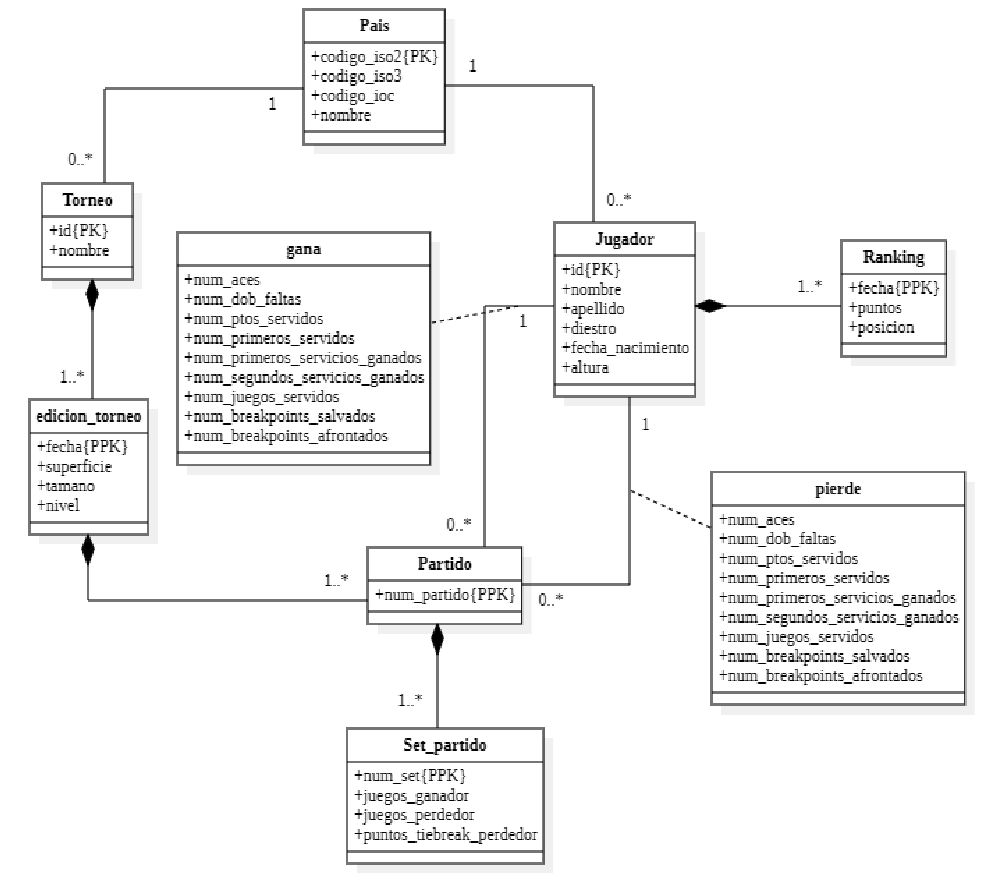
\includegraphics[width=0.7\textwidth]{fotos/esquema.png}
  \caption{Esquema de la base de datos de partidos de tenis.}
  \label{fig:schbd}
\end{figure}

En la figura \ref{fig:schbd} se muestra el esquema de la base de datos de partidos de tenis. Comenzaremos explicando este esquema de forma breve, pero haciendo especial hincapié en las relaciones entre las distintas tablas, ya que esto ayudará a comprender mejor las condiciones de \textit{join} a usar en las consultas que usen este esquema. Destacamos que no se hará uso de la tabla \texttt{ranking}, por lo que no se comentará en el siguiente análisis. \\

La tabla \texttt{pais} contiene la información relativa a países, y se usará tanto para mostrar el país dónde se celebra un torneo como para referenciar el país de procedencia de un jugador; su clave primaria es \texttt{codigo\_iso2}. La tabla \texttt{jugador} contiene la información de los jugadores, y su clave primaria es el \texttt{id} de cada jugador; el atributo \texttt{pais} referencia a \texttt{pais(codigo\_iso2)}. La tabla \texttt{torneo} contiene la información de los torneos; su clave primaria es el \texttt{id} de cada torneo y el atributo \texttt{pais} referencia a \texttt{pais(codigo\_iso2)}. La tabla \texttt{edicion\_torneo} contiene la información de las ediciones de los torneos; su clave primaria es una combinación de los atributos \texttt{torneo} y \texttt{fecha}, donde el atributo \texttt{torneo} es una referencia a \texttt{torneo(id)}. La tabla \texttt{partido} contiene la información de los partidos disputados; su clave primaria es la combinación de los atributos \texttt{torneo}, \texttt{fecha} y \texttt{num\_partido}, y tiene una clave foránea compuesta por los atributos \texttt{torneo} y \texttt{fecha}, que referencia a la clave primaria de \texttt{edicion\_torneo}, \texttt{edicion\_torneo(torneo, fecha)}. Además, los atributos \texttt{ganador} y \texttt{perdedor} son los \texttt{id} de los jugadores, por lo que puede enlazarse esta tabla con la de \texttt{jugador} mediante \texttt{jugador(id)}. Por último, la tabla \texttt{sets\_partido} contiene la información de los sets de los partidos; su clave primaria es la combinación de los atributos \texttt{torneo}, \texttt{fecha}, \texttt{num\_partido} y \texttt{num\_set}, y tiene una clave foránea compuesta por los atributos \texttt{torneo}, \texttt{fecha} y \texttt{num\_partido}, que referencia a la clave primaria de \texttt{partido}, \texttt{partido(torneo, fecha, num\_partido)}. \\

Tras ver cómo se estructura la base de datos a usar, creamos la base de datos en PostgreSQL y cargamos los datos en ella. La estructura relacional se proporciona en el archivo \texttt{schema.sql}, y los datos en los archivos \texttt{pais.csv}, \texttt{jugador.csv}, \texttt{torneo.csv}, \texttt{edicion\_torneo.csv}, \texttt{partido.csv}, \texttt{sets\_partido.csv} y \texttt{ranking.csv}. Una vez creada la base de datos \texttt{tenis}, ejecutamos el archivo \texttt{schema.sql} con la definición de los esquemas de las tablas mediante el siguiente comando en la terminal:

\begin{lstlisting}[style=terminal]
psql -U alumnogreibd -d tenis -f /home/alumnogreibd/BDGE/datos/datos_tenis/schema.sql
\end{lstlisting}

Ahora, con los esquemas definidos (pero vacíos), cargamos los datos a partir de los archivos \texttt{.csv} con los siguientes comandos en terminal (es importante seguir el orden de carga de los datos debido a las dependencias entre las tablas):

\begin{lstlisting}[style=terminal]
psql -U alumnogreibd -d tenis -c "\copy pais from /home/alumnogreibd/BDGE/datos/datos_tenis/pais.csv csv"
psql -U alumnogreibd -d tenis -c "\copy jugador from /home/alumnogreibd/BDGE/datos/datos_tenis/jugador.csv csv"
psql -U alumnogreibd -d tenis -c "\copy torneo from /home/alumnogreibd/BDGE/datos/datos_tenis/torneo.csv csv"
psql -U alumnogreibd -d tenis -c "\copy edicion_torneo from /home/alumnogreibd/BDGE/datos/datos_tenis/edicion_torneo.csv csv"
psql -U alumnogreibd -d tenis -c "\copy partido from /home/alumnogreibd/BDGE/datos/datos_tenis/partido.csv csv"
psql -U alumnogreibd -d tenis -c "\copy sets_partido from /home/alumnogreibd/BDGE/datos/datos_tenis/sets_partido.csv csv"
psql -U alumnogreibd -d tenis -c "\copy ranking from /home/alumnogreibd/BDGE/datos/datos_tenis/ranking.csv csv"
\end{lstlisting}

Este orden es lógico por las dependencias entre tablas que comentamos anteriormente: \texttt{sets\_partido} referencia a \texttt{partido}, por lo que es necesario cargar primero los datos de \texttt{partido} para poder cargar los de \texttt{sets\_partido}. Este razonamiento aplica al resto de tablas: \texttt{partido} referencia a \texttt{edicion\_torneo}, que referencia a \texttt{torneo}, que a su vez referencia a \texttt{pais}, que es referenciado por \texttt{jugador}. \\

En las siguientes consultas, los \textit{join} se harán mediante \textit{theta join} (\textit{inner} por defecto). En caso de que se quiera hacer otro tipo de \textit{join}, se especificará de forma clara en la consulta. Esto considera el producto cartesiano de las tablas a unir y selecciona solo las tuplas que verifiquen el predicado (la condición o condiciones de \textit{join}). Estos \textit{join} se harán de forma general de forma implícita en la claúsula \texttt{where}, siguiendo los atributos referenciados entre las tablas. El \texttt{where} hace una selección de tuplas (filas) que cumplen el predicado o los predicados mencionados. Teniendo esto muy presente, abusaremos un poco del lenguaje para ser más concisos y frases como: ``seleccionamos solo las tuplas en las que un jugador concreto es el ganador del partido'', reformularemos como ``seleccionamos los partidos que ganó un jugador concreto''. \\


\subsubsection{Muestra todos los ganadores del torneo ``Wimbledon'' (Nombre, apellidos y año). Ordena el resultado por año.}

Para esta consulta necesitamos la información de los jugadores, los partidos y los torneos, por lo que comenzamos en el \texttt{from} con el producto cartesiano de las tablas \texttt{jugador}, \texttt{partido} y \texttt{torneo} (especificando un alias para cada una de ellas). A continuación, especificamos las condiciones de \textit{join} en el \texttt{where}, así como otras condiciones de selección: 
\begin{itemize}
\item Condiciones de \textit{join}:
\begin{itemize}
\item El predicado \texttt{j.id = p.ganador} sirve para unir la tabla \texttt{jugador} con la tabla \texttt{partido} mediante el atributo \texttt{id} de la tabla \texttt{jugador} y el atributo \texttt{ganador} de la tabla \texttt{partido}, haciendo una selección únicamente de las tuplas que cumplan esta condición. Esto nos permite, para cada jugador, seleccionar solo los partidos en los que ha ganado.
\item El predicado \texttt{t.id = p.torneo} sirve para unir la tabla \texttt{torneo} con la tabla \texttt{partido} mediante el atributo \texttt{id} de la tabla \texttt{torneo} y el atributo \texttt{torneo} de la tabla \texttt{partido}, haciendo una selección únicamente de las tuplas que cumplan esta condición. Esto nos permite seleccionar solo los partidos que se han jugado en un torneo concreto.
\end{itemize}
\item Condiciones de selección:
\begin{itemize}
\item La condición \texttt{t.nombre = `Wimbledon'} selecciona solo el torneo cuyo nombre es ``Wimbledon''. Al hacer el \textit{join} con la tabla \texttt{torneo}, estamos seleccionando solo los partidos que se han jugado en el torneo ``Wimbledon''.
\item La condición \texttt{p.ronda = `F'} selecciona solo los partidos que han sido finales.
\end{itemize}
\end{itemize}

Tras seleccionar las tuplas que nos interesan, usamos el \texttt{select} para obtener la proyección de las filas que nos interesan: en esta caso, nos quedamos con los atributos \texttt{nombre} y \texttt{apellido} de la tabla \texttt{jugador} y el año de la fecha del partido, que denotaremos por el alias ``ano''. Como \texttt{p.fecha} es del tipo \texttt{date}, este último atributo lo obtenemos mediante la función \texttt{extract()}, especificando que solo queremos el año de ese atributo (\texttt{year from p.fecha}). Tras esto, ordenamos el resultado por año con \texttt{order by ano}; el orden por defecto es ascendente. El código de la consulta se muestra a continuación, y el resultado se pueden ver en la figura \ref{fig:q1_rel}.

\begin{minted}[frame=single, fontsize=\footnotesize]{sql}
select j.nombre, j.apellido, extract(year from p.fecha) as ano
from jugador j, partido p, torneo t
where j.id = p.ganador 
  and t.id = p.torneo 
  and t.nombre = 'Wimbledon' 
  and p.ronda = 'F'
order by ano
\end{minted}

\begin{figure}[H]
\centering
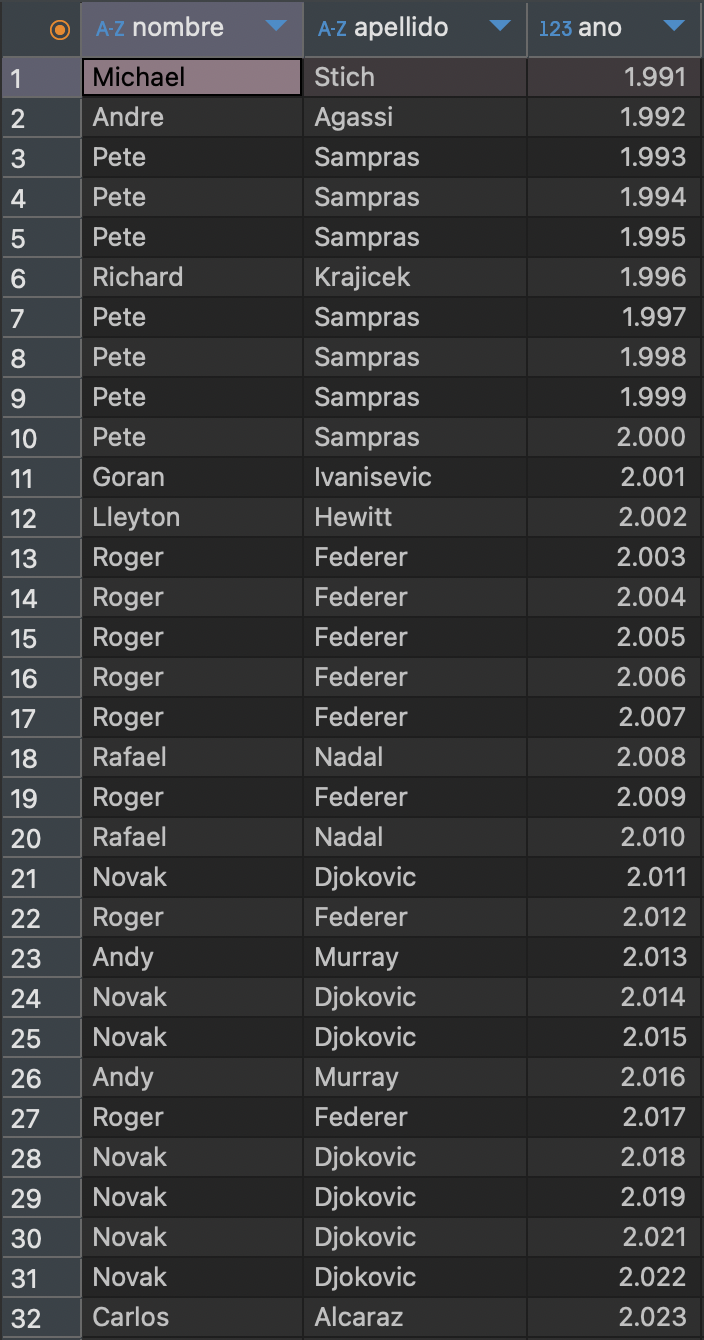
\includegraphics[height=0.4\textheight]{fotos/q1_rel.png}
\caption{Modelo relacional Postgresql, consulta 1.}
\label{fig:q1_rel}
\end{figure}



\subsubsection{Muestra los años en los que Roger Federer ganó algún torneo de nivel Gran Slam (G) o Master 1000 (M). Para cada año, muestra el número de torneos y lista sus nombres (ordenados por la fecha de celebración). Ordena el resultado por el año}

Para esta consulta necesitamos información de los jugadores, los partidos, los torneos y las ediciones de los torneos. Comenzamos en el \texttt{from} con el producto cartesiano de las tablas \texttt{jugador}, \texttt{partido}, \texttt{torneo} y \texttt{edicion\_torneo} (especificando un alias para cada una de ellas). A continuación, especificamos las condiciones de \textit{join} en el \texttt{where}, así como otras condiciones de selección:
\begin{itemize}
\item Condiciones de \textit{join} que, en global, nos permitirán seleccionar las tuplas de un jugador específico que ganó un torneo específico en un año específico:
\begin{itemize}
\item El predicado \texttt{j.id = p.ganador} sirve para unir la tabla \texttt{jugador} con la tabla \texttt{partido} mediante el atributo \texttt{id} de la tabla \texttt{jugador} y el atributo \texttt{ganador} de la tabla \texttt{partido}, haciendo una selección únicamente de las tuplas que cumplan esta condición. Esto nos permite, para cada jugador, seleccionar solo los partidos en los que ha ganado.
\item El predicado \texttt{t.id = p.torneo} sirve para unir la tabla \texttt{torneo} con la tabla \texttt{partido} mediante el atributo \texttt{id} de la tabla \texttt{torneo} y el atributo \texttt{torneo} de la tabla \texttt{partido}, haciendo una selección únicamente de las tuplas que cumplan esta condición. Esto nos permite seleccionar solo los partidos que se han jugado en un torneo concreto.
\item El predicado \texttt{t.id = et.torneo} sirve para unir la tabla \texttt{torneo} con la tabla \texttt{edicion\_torneo} mediante el atributo \texttt{id} de la tabla \texttt{torneo} y el atributo \texttt{torneo} de la tabla \texttt{edicion\_torneo}, haciendo una selección únicamente de las tuplas que cumplan esta condición. Esto nos permite seleccionar ediciones de torneos concretos.
\item El predicado \texttt{p.fecha = et.fecha} sirve para unir la tabla \texttt{partido} con la tabla \texttt{edicion\_torneo} mediante el atributo \texttt{fecha} de la tabla \texttt{partido} y el atributo \texttt{fecha} de la tabla \texttt{edicion\_torneo}, haciendo una selección únicamente de las tuplas que cumplan esta condición. Esto nos permite seleccionar solo los partidos que se han jugado en una edición concreta de un torneo (concreto, por la condición anterior).
\end{itemize}
\item Estamos interesados específicamente en torneos de nivel Gran Slam (G) o Master 1000 (M) y en las finales ganadas por Roger Federer (lo que indica que ganó el torneo) durante varios años (es decir, varias ediciones de torneos). Por tanto, las condiciones de selección son:
\begin{itemize}
\item El predicado \texttt{p.ronda = 'F'} selecciona solo los partidos que han sido finales.
\item El predicado \texttt{j.nombre = 'Roger' and j.apellido = 'Federer'} selecciona solo los partidos en los que ha ganado ``Roger Federer''.
\item El predicado \texttt{et.nivel in ('G', 'M')} selecciona solo los torneos de nivel Gran Slam (G) o Master 1000 (M).
\end{itemize}
\end{itemize}

Con el \texttt{group by} agrupamos los resultados por el año en que se celebraron los torneos, para su posterior concatenación. Por último, obtenemos la proyección de los atributos que nos interesan: el año, que lo obtenemos extrayendo el año de la fecha de celebración del partido; el número de torneos ganados, que lo obtenemos contando el número de torneos distintos (usamos el \texttt{id} del torneo para diferenciar) en el resultado agrupado por año (\texttt{count(distinct t.id)}). Como última proyección, obtenemos una concantenación (con \texttt{string\_agg()}) de esos torneos, separados por comas y ordenados por fecha de celebración de esa edición, en orden ascendente (\texttt{order by et.fecha}). El código de la consulta se muestra a continuación, y el resultado se pueden ver en la figura \ref{fig:q2_rel}.

\begin{minted}[frame=single, fontsize=\footnotesize]{sql}
select extract(year from et.fecha) as ano, count(distinct t.id) as numero_torneos, 
	string_agg(t.nombre, ', ' order by et.fecha) as torneos
from jugador j, partido p, torneo t, edicion_torneo et
where j.id = p.ganador
  and t.id = et.torneo
  and p.torneo = t.id
  and p.fecha = et.fecha
  and p.ronda = 'F'
  and j.nombre = 'Roger'
  and j.apellido = 'Federer'
  and et.nivel in ('G', 'M')
group by ano
\end{minted}

\begin{figure}[H]
\centering
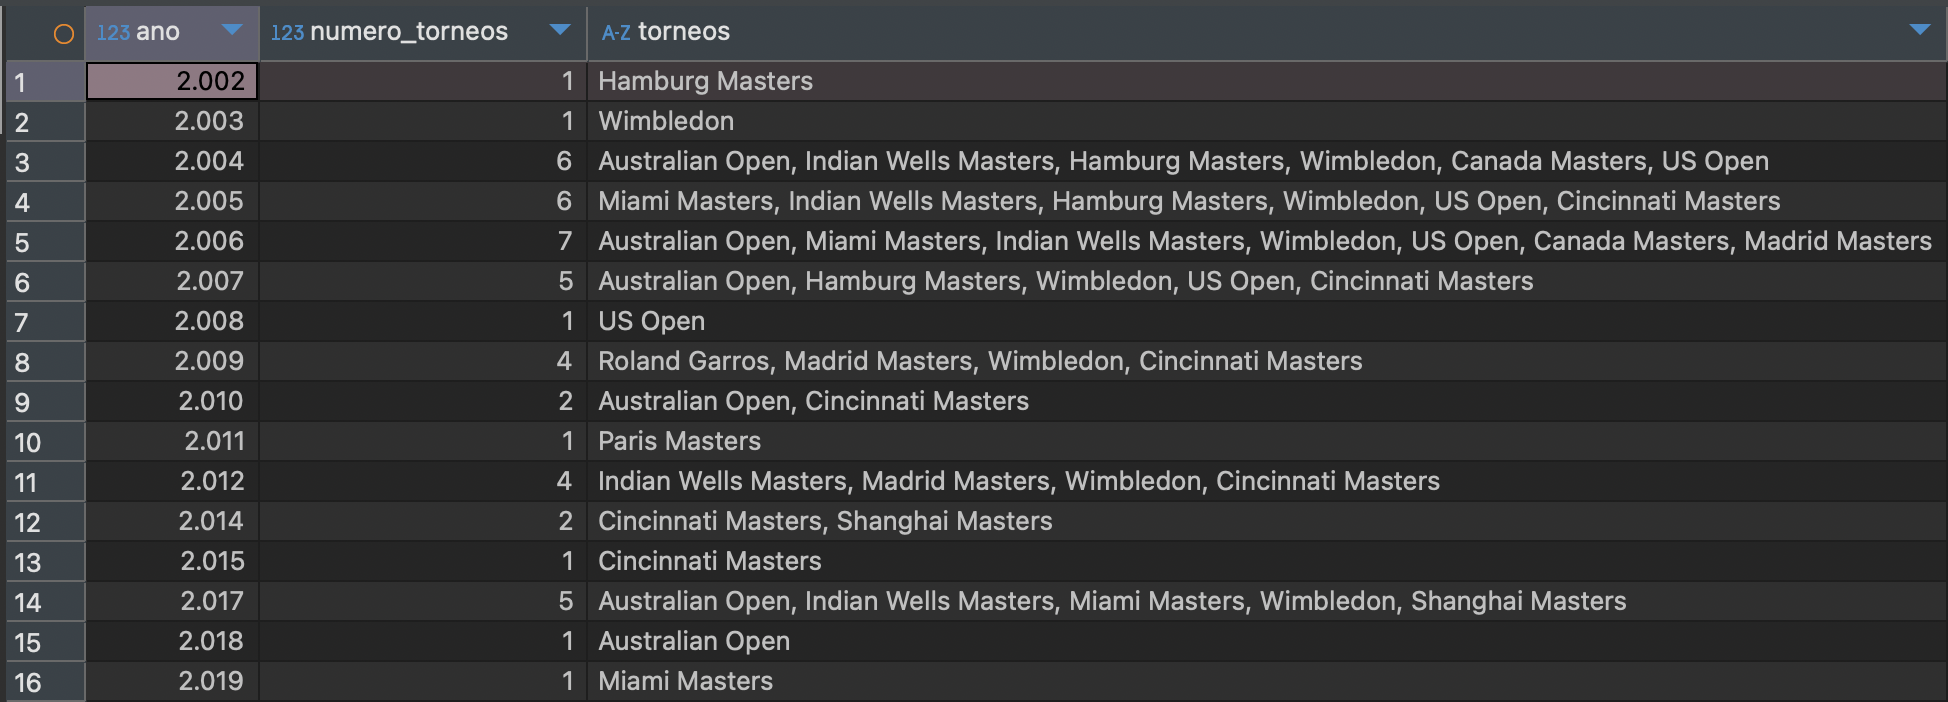
\includegraphics[width=0.8\textwidth]{fotos/q2_rel.png}
\caption{Modelo relacional Postgresql, consulta 2.}
\label{fig:q2_rel}
\end{figure}


\subsubsection{Muestra los partidos de semifinales (ronda='SF') y final (ronda = 'F') del torneo de "Roland Garros" del 2018. Para cada partido muestra la ronda, el tipo de desenlace, el nombre y apellidos del ganador y el nombre y apellidos del perdedor y el resultado con el número de juegos del ganador y del perdedor en cada set, y opcionalmente en paréntesis el número de juegos del perdedor en el tie break}

Para esta consulta necesitamos información de los partidos, los jugadores, los torneos y los sets de los partidos; como debemos distinguir entre el ganador y el perdedor, sin ningún tipo de ambigüedad, en el \texttt{from} usamos dos instancias de la tabla \texttt{jugador}, cada una con un alias distinto, por lo que estaremos haciendo el producto cartesiano de la tabla \texttt{jugador} consigo misma, así como con las tablas \texttt{partido}, \texttt{torneo} y \texttt{sets\_partido} (especificando un alias para cada una de ellas). A continuación, especificamos las condiciones de \textit{join} en el \texttt{where}, así como otras condiciones de selección:
\begin{itemize}
\item Condiciones de \textit{join} que, en global, nos permitirán seleccionar las tuplas de partidos específicos de un torneo específico en una fecha específica:
\begin{itemize}
\item El predicado \texttt{jg.id = p.ganador} sirve para unir la tabla \texttt{jugador} con la tabla \texttt{partido} mediante el atributo \texttt{id} de la tabla \texttt{jugador} y el atributo \texttt{ganador} de la tabla \texttt{partido}, haciendo una selección únicamente de las tuplas que cumplan esta condición. Esto nos permite, para cada jugador, seleccionar solo los partidos en los que ha ganado.
\item Del mismo modo, usamos el predicado \texttt{jp.id = p.perdedor} para eleccionar solo los partidos en los que ha perdido un determinado jugador. 
\item El predicado \texttt{p.fecha = sp.fecha} sirve para unir la tabla \texttt{partido} con la tabla \texttt{sets\_partido} mediante el atributo \texttt{fecha} de la tabla \texttt{partido} y el atributo \texttt{fecha} de la tabla \texttt{sets\_partido}, haciendo una selección únicamente de las tuplas que cumplan esta condición. Esto nos permite seleccionar solo los sets de los partidos que se han jugado en una fecha concreta.
\item Como la fecha anterior no es unívoca para cada partido, necesitamos una condición adicional para obtener los sets de un partido determinado. Para ello, usamos el predicado \texttt{p.num\_partido = sp.num\_partido}, que une la tabla \texttt{partido} con la tabla \texttt{sets\_partido} mediante el atributo \texttt{num\_partido} de la tabla \texttt{partido} y el atributo \texttt{num\_partido} de la tabla \texttt{sets\_partido}, haciendo una selección únicamente de las tuplas que cumplan esta condición.
\item El predicado \texttt{t.id = p.torneo} sirve para unir la tabla \texttt{torneo} con la tabla \texttt{partido} mediante el atributo \texttt{id} de la tabla \texttt{torneo} y el atributo \texttt{torneo} de la tabla \texttt{partido}, haciendo una selección únicamente de las tuplas que cumplan esta condición. Esto nos permite seleccionar solo los partidos que se han jugado en un torneo concreto.
\end{itemize}
\item Concretamente, estamos interesados en las semifinales (ronda='SF') y la final (ronda='F) del torneo de ``Roland Garros'' del 2018. Por tanto, las condiciones de selección son:
\begin{itemize}
\item El predicado \texttt{p.ronda in ('SF', 'F')} selecciona solo los partidos que han sido semifinales o finales.
\item El predicado \texttt{t.nombre = 'Roland Garros'} selecciona solo los partidos que se han jugado en el torneo ``Roland Garros''.
\item El predicado \texttt{extract(year from p.fecha) = '2018'} selecciona solo los partidos que se han jugado en el año 2018.
\end{itemize}
\end{itemize}

Ahora, para cada combinación de \texttt{p.ronda}, \texttt{p.desenlace}, \texttt{jg.nombre}, \texttt{jg.apellido}, \texttt{jp.nombre} y \texttt{jp.apellido}, tendremos una fila para cada set, donde solo variará la información de los juegos ganados y perdidos. Por tanto, agrupamos por los atributos mencionados anteriormente y, en la proyección, concatenamos los resultados de los juegos ganados y perdidos en cada set, así como el resultado final del partido, para lo que usamos la función \texttt{string\_agg()}. Como también debemos especificar la puntuación del \textit{tiebreak} (en caso de haberla), usamos un \texttt{case} para comprobar si el atributo \texttt{puntos\_tiebreak\_perdedor} es \texttt{null} o no: en caso que sea nulo, concatenamos una cadena vacia, en caso de no ser nulo, concatenamos la puntuación del \textit{tiebreak}, puesta entre paréntesis. Si bien esta es una parte de la proyección, el resto incluye simplemente la ronda, el desenlace, la fecha y los nombres y apellidos de los jugadores concatenados (un atributo para el ganador y otro para el perdedor). El código de la consulta se muestra a continuación, y el resultado se pueden ver en la figura \ref{fig:q3_rel}.

\begin{minted}[frame=single, fontsize=\footnotesize]{sql}
select p.ronda, p.desenlace, jg.nombre || ' ' || jg.apellido AS ganador, 
	jp.nombre || ' ' || jp.apellido AS perdedor, 
	STRING_AGG(sp.juegos_ganador || '-' || sp.juegos_perdedor ||
		case
		  when sp.puntos_tiebreak_perdedor is not null then 
		  	'(' || sp.puntos_tiebreak_perdedor || ')'
		  else 
		  	'' 
		end, ', ' order by sp.num_set) as resultado
from partido p, jugador jg, jugador jp, sets_partido sp, torneo t
where jg.id = p.ganador
  and jp.id = p.perdedor
  and p.fecha = sp.fecha
  and p.num_partido = sp.num_partido
  and t.id = p.torneo
  and p.ronda in ('SF', 'F')
  and t.nombre = 'Roland Garros'
  and extract(year from p.fecha) = '2018'
group by p.ronda, p.desenlace, jg.nombre, jg.apellido, jp.nombre, jp.apellido
\end{minted}

\begin{figure}[H]
\centering
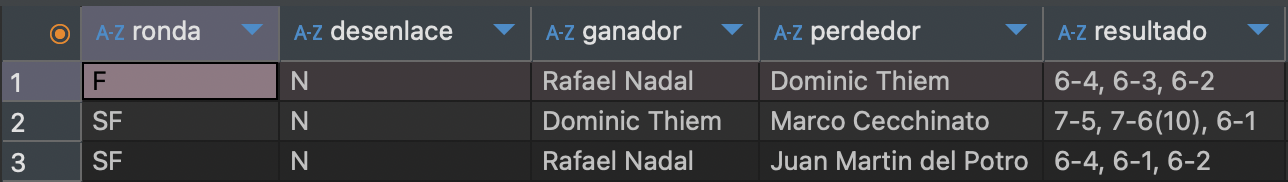
\includegraphics[width=0.7\textwidth]{fotos/q3_rel.png}
\caption{Modelo relacional Postgresql, consulta 3.}
\label{fig:q3_rel}
\end{figure}

\subsubsection{Muestra la lista de jugadores españoles (ES) que ganaron algún torneo de nivel Gran Slam (G). Para cada jugador muestra los siguientes datos resumen de todos sus partidos: número de partidos jugados, porcentaje de victorias, porcentaje de aces, porcentaje de dobles faltas, porcentaje de servicios ganados, porcentaje de restos ganados, porcentaje de break points salvados (de los sufridos en contra), porcentaje de break points ganados (de los provocados a favor)}

Esta consulta la dividiremos en dos partes: primero, buscaremos los jugadores españoles que ganaron algún torneo de nivel Grand Slam (G), y, a continuación, calcularemos los datos resumen que se piden de todos sus partidos. Para la primera parte, necesitamos información de los jugadores, los partidos y las ediciones de los torneos; comenzamos en el \texttt{from} con el producto cartesiano de las tablas \texttt{jugador}, \texttt{partido} y \texttt{edicion\_torneo} (especificando un alias para cada una de ellas). A continuación, especificamos las condiciones de \textit{join} en el \texttt{where}, así como otras condiciones de selección:
\begin{itemize}
\item Condiciones de \textit{join} que, en global, nos permitirán seleccionar las tuplas de un torneo específico:
\begin{itemize}
\item El predicado \texttt{j.id = p.ganador} sirve para unir la tabla \texttt{jugador} con la tabla \texttt{partido} mediante el atributo \texttt{id} de la tabla \texttt{jugador} y el atributo \texttt{ganador} de la tabla \texttt{partido}, haciendo una selección únicamente de las tuplas que cumplan esta condición. Esto nos permite, para cada jugador, seleccionar solo los partidos en los que ha ganado. 
\item El predicado \texttt{p.torneo = et.torneo} sirve para unir la tabla \texttt{partido} con la tabla \texttt{edicion\_torneo} mediante el atributo \texttt{torneo} de la tabla \texttt{partido} y el atributo \texttt{torneo} de la tabla \texttt{edicion\_torneo}, haciendo una selección únicamente de las tuplas que cumplan esta condición. Esto nos permite seleccionar solo los partidos que se han jugado en una edición concreta de un torneo.
\item El predicado \texttt{p.fecha = et.fecha} sirve para unir la tabla \texttt{partido} con la tabla \texttt{edicion\_torneo} mediante el atributo \texttt{fecha} de la tabla \texttt{partido} y el atributo \texttt{fecha} de la tabla \texttt{edicion\_torneo}, haciendo una selección únicamente de las tuplas que cumplan esta condición. Esto nos permite seleccionar solo los partidos que se han jugado en una fecha concreta.
\end{itemize}
\item Como de todo lo anterior solo nos interesan los partidos finales (F) de torneos de nivel Grand Slam (G) y ganados por jugadores españoles (ES), las condiciones de selección son:
\begin{itemize}
\item El predicado \texttt{p.ronda = `F'} selecciona solo los partidos que han sido finales.
\item El predicado \texttt{et.nivel = `G'} selecciona solo los torneos de nivel Grand Slam (G).
\item El predicado \texttt{j.pais = `ES'} selecciona solo los jugadores españoles.
\end{itemize}
\end{itemize}

Con todo esto, obtenemos una tabla con los jugadores españoles que han ganado algún torneo de nivel Grand Slam (G), pero hay repeticion ya que estamos considerando cada edición de cada Grand Slam. Para quedarnos solo con el subconjunto que nos interesa (sin repetición), usamos un \texttt{distinct} en la proyección. Concretamente, obtenemos la proyección del \texttt{id} y el nombre completo del jugador, que concatenamos con el operador \texttt{||}, y aplicamos el \texttt{distinct} sobre la proyección. Esta tabla resultado la guardamos como \texttt{jugadores\_espanoles\_ganadores}, y la usaremos en la segunda parte de la consulta. \\

Para obtener las estadísticas resumen de cada jugador español ganador de un Grand Slam, necesitamos solo información sobre quiénes son esos jugadores y sobre los partidos que han jugado. Por tanto, en el \texttt{from} usamos la tabla \texttt{jugadores\_espanoles\_ganadores} que acabamos de crear, y la tabla \texttt{partido} (especificando un alias para cada una de ellas). A continuación, especificamos las condiciones de \textit{join} en el \texttt{where}, así como otras condiciones de selección:
\begin{itemize}
\item Condiciones de \textit{join} que, en global, nos permitirán seleccionar las tuplas de partidos de un jugador específico:
\begin{itemize}
\item El predicado \texttt{jeg.id\_jugador = p.ganador or jeg.id\_jugador = p.perdedor} nos permite seleccionar los partidos, tanto ganados como perdidos, en los que ha participado un jugador específico de la tabla \texttt{jugadores\_espanoles\_ganadores}.
\end{itemize}
\end{itemize}

Con esto, obtenemos una fila por cada partido de cada jugador, por lo que agrupamos por el jugador con \texttt{group by} antes de agregar valores. En la proyección, obtenemos varios atributos, que redondearemos a un decimal usando \texttt{round(\dots, 1)}. En general, excepto para los partidos y el porcentaje de victorias, todas las estadísticas se calculan de la misma forma cosniderando atributos distintos; por ello, daremos una explicación detallada de una de ellas, y el resto simplemente mencionaremos qué atributos hemos usado y si se siguió un proceso distinto.
\begin{itemize}
\item El nombre completo del jugador, que concatenamos previamente con el operador \texttt{||}.
\item El número de partidos jugados como el conteo de los partidos en los que ha participado \\ (\texttt{count(p.num\_partido)}).
\item El porcentaje de victorias, que calculamos como el número de partidos ganados entre el número total de partidos jugados, multiplicado por 100. Para obtener el número de partidos ganados, usamos un \texttt{case} que comprueba si el jugador es el ganador del partido o no. Esto genera una lista que contiene 1 si el jugador es el ganador y 0 si no lo es, y con \texttt{sum()} sumamos los valores de esta lista para obtener el número de partidos ganados. 
\item El porcentaje de aces, que calculamos como el número de aces del jugador entre el número total de puntos servidos, multiplicado por 100. Para obtener el número de aces, simplemente sumamos (\texttt{sum()}) los valores la columna \texttt{num\_aces\_ganador} o \texttt{num\_aces\_perdedor} para el jugador específico. El número de puntos servidos lo obtenemos de forma análoga usando la columna \texttt{num\_ptos\_servidos\_ganador} o \texttt{num\_ptos\_servidos\_perdedor} según corresponda. Para ver si corresponde usar las estadísticas del ganador o del perdedor, se considerará un \texttt{case} que distinga si nuestro jugador está en la posición de ganador o perdedor, y se usarán las estadísticas correspondientes. Además, se implementará la función \texttt{nullif()} para gestionar las divisiones por 0. 
\item El porcentaje de dobles faltas, que calculamos de forma análoga al porcentaje de aces, pero usando las columnas \texttt{num\_dob\_faltas\_ganador} y \texttt{num\_dob\_faltas\_perdedor} en lugar de las columnas de aces. 
\item El porcentaje de servicios ganados, que calculamos de forma análoga al porcentaje de aces, pero usando una suma de las columnas \texttt{num\_primeros\_servicios\_ganados\_ganador} y \texttt{num\_segundos\_servicios\_gan-}\\\texttt{ados\_ganador}, o de \texttt{num\_primeros\_servicios\_ganados\_perdedor} y \texttt{num\_segundos\_servicios\_ganados}\\\texttt{\_perdedor} en lugar de las columnas de aces.
\item El porcentaje de restos ganados, que calculamos de forma análoga al porcentaje de aces. Sin embargo, está vez usaremos las estadísticas de rival para obtener la del jugador que nos interesa: si nuestro jugador ganó, nos fijaremos en \texttt{num\_ptos\_servidos\_perdedor} y \texttt{num\_restos\_ganados\_perdedor}, y si perdió, en \texttt{num\_ptos\_servidos\_perdedor}, \texttt{num\_primeros\_servicios\_ganados\_perdedor} y \texttt{p.num\_segundos\_servi-} \\ \texttt{cios\_ganados\_perdedor}, y si perdió, en los mismos atributos pero del ganador. El porcentaje de restos ganados por nuestro jugador será entonces el cociente entre el número de saques que su rival no consiguió ganar el servicio, que lo obtenemos como la resta entre los puntos servidos y los primeros y segundos servicios ganados, y el número total de puntos servidos por el rival, multiplicado por 100.
\item El porcentaje de \textit{breaks} salvados, que calculamos de forma análoga al porcentaje de aces pero usando las columnas \texttt{num\_break\_salvados\_ganador} o \texttt{num\_break\_salvados\_perdedor} en lugar de las columnas de aces, y \texttt{num\_break\_afrontados\_ganador} o \texttt{num\_break\_afrontados\_perdedor} en lugar de las columnas de puntos servidos.
\item El porcentaje de \textit{breaks} ganados, que calculamos de forma análoga al porcentaje de aces pero usando las estadísticas del rival. Lo obtenemos como el cociente entre la el número de \textit{breaks} que perdió el rival (calculado como la diferencia entre afrontados y ganados) y el número total de \textit{breaks} que afrontó el rival, multiplicado por 100.
\end{itemize}

\noindent A continuación se muestra la consulta completa y el resultado se puede ver en la figura \ref{fig:q4_rel}.

\begin{minted}[frame=single, fontsize=\footnotesize]{sql}
with jugadores_espanoles_ganadores as (
    select distinct j.id as id_jugador, j.nombre || ' ' || j.apellido as jugador
    from partido p, jugador j, edicion_torneo et 
    where p.ganador = j.id 
        and p.torneo = et.torneo 
        and p.fecha = et.fecha
        and j.pais = 'ES'
        and p.ronda = 'F'
        and et.nivel = 'G'
)

select jeg.jugador, count(p.num_partido) as partidos,
    round(100.0 * sum(case when jeg.id_jugador = p.ganador then 1 else 0 end) / 
		count(p.num_partido), 1) as pcje_victorias, 
    round(100.0 * sum(case when jeg.id_jugador = p.ganador then 
		p.num_aces_ganador else p.num_aces_perdedor end) / 
        nullif(sum(case when jeg.id_jugador = p.ganador then p.num_ptos_servidos_ganador 
		else p.num_ptos_servidos_perdedor end), 0), 1) as pcje_aces, 
    round(100.0 * sum(case when jeg.id_jugador = p.ganador then p.num_dob_faltas_ganador 
		else p.num_dob_faltas_perdedor  end) / 
        nullif(sum(case when jeg.id_jugador = p.ganador then p.num_ptos_servidos_ganador 
		else p.num_ptos_servidos_perdedor end), 0), 1) as pcje_dobles_faltas, 
    round(100.0 * sum(case when jeg.id_jugador = p.ganador then 
		p.num_primeros_servicios_ganados_ganador + p.num_segundos_servicios_ganados_ganador 
        else p.num_primeros_servicios_ganados_perdedor + p.num_segundos_servicios_ganados_perdedor end) / 
        nullif(sum(case when jeg.id_jugador = p.ganador then p.num_ptos_servidos_ganador 
		else p.num_ptos_servidos_perdedor end), 0), 1) as pcje_servicios_ganados, 
    round(100.0 * sum(case when jeg.id_jugador = p.ganador then 
		p.num_ptos_servidos_perdedor - p.num_primeros_servicios_ganados_perdedor - 
		p.num_segundos_servicios_ganados_perdedor 
        else p.num_ptos_servidos_ganador - p.num_primeros_servicios_ganados_ganador - 
		p.num_segundos_servicios_ganados_ganador end) / 
        nullif(sum(case when jeg.id_jugador = p.ganador then p.num_ptos_servidos_perdedor 
		else p.num_ptos_servidos_ganador end), 0), 1) as pcje_restos_ganados,
    round(100.0 * sum(case when jeg.id_jugador = p.ganador then p.num_break_salvados_ganador 
		else p.num_break_salvados_perdedor end) / 
        nullif(sum(case when jeg.id_jugador = p.ganador then p.num_break_afrontados_ganador 
		else p.num_break_afrontados_perdedor end), 0), 1) as pcje_breaks_salvados, 
    round(100.0 * sum(case when jeg.id_jugador = p.ganador then 
		p.num_break_afrontados_perdedor - p.num_break_salvados_perdedor 
        else p.num_break_afrontados_ganador - p.num_break_salvados_ganador end) / 
        nullif(sum(case when jeg.id_jugador = p.ganador then p.num_break_afrontados_perdedor 
		else p.num_break_afrontados_ganador end), 0), 1) as pcje_breaks_ganados
from jugadores_espanoles_ganadores jeg, partido p
where jeg.id_jugador = p.ganador 
	or jeg.id_jugador = p.perdedor
group by jeg.jugador
\end{minted}

\begin{figure}[H]
\centering
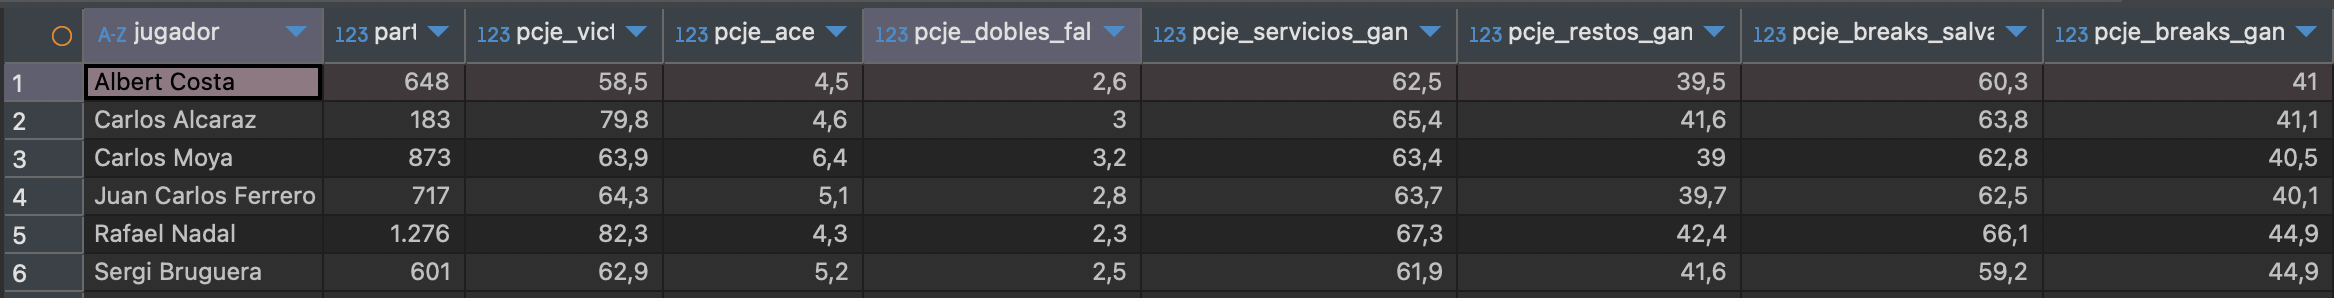
\includegraphics[width=\textwidth]{fotos/q4_rel.png}
\caption{Modelo relacional Postgresql, consulta 4.}
\label{fig:q4_rel}
\end{figure}

\subsubsection{Lista los jugadores que fueron derrotados (en algún partido del 2018) por el rival de Rafael Nadal de la primera ronda (R128) de Roland Garros de 2018}

Esta consulta la dividiremos de nuevo en dos partes. Primero, buscaremos el rival de Rafael Nadal en la primera ronda de Roland Garros de 2018, y, a continuación, buscaremos los jugadores que fueron derrotados por ese rival en algún partido de 2018. Para la primera parte, necesitamos información de los partidos, los jugadores, los torneos y sus ediciones; comenzamos en el \texttt{from} con el producto cartesiano de las tablas \texttt{jugador}, \texttt{partido}, \texttt{torneo} y \texttt{edicion\_torneo} (especificando un alias para cada una de ellas) Aquí, de nuevo, usamos la tabla \texttt{jugador} dos veces, una para identificar a un jugador (que será Rafael Nadal) y otra para identificar al rival sin ambigüedad. A continuación, especificamos las condiciones de \textit{join} en el \texttt{where}, así como otras condiciones de selección:
\begin{itemize}
\item Condiciones de \textit{join} que, en global, nos permitirán seleccionar las tuplas de partidos específicos:
\begin{itemize}
\item El predicado \texttt{jg.id = p.ganador} sirve para unir la tabla \texttt{jugador} con la tabla \texttt{partido} mediante el atributo \texttt{id} de la tabla \texttt{jugador} y el atributo \texttt{ganador} de la tabla \texttt{partido}, haciendo una selección únicamente de las tuplas que cumplan esta condición. Esto nos permite seleccionar solo los partidos en los que ganó un jugador concreto.
\item El predicado \texttt{jp.id = p.perdedor} sirve para unir la tabla \texttt{jugador} con la tabla \texttt{partido} mediante el atributo \texttt{id} de la tabla \texttt{jugador} y el atributo \texttt{perdedor} de la tabla \texttt{partido}, haciendo una selección únicamente de las tuplas que cumplan esta condición. Esto nos permite seleccionar solo los partidos en los que un jugador concreto es el perdedor del partido.
\item El predicado \texttt{p.torneo = et.torneo} sirve para unir la tabla \texttt{partido} con la tabla \texttt{edicion\_torneo} mediante el atributo \texttt{torneo} de la tabla \texttt{partido} y el atributo \texttt{torneo} de la tabla \texttt{edicion\_torneo}, haciendo una selección únicamente de las tuplas que cumplan esta condición. Esto nos permite seleccionar solo los partidos que se han jugado en una edición concreta de un torneo.
\item El predicado \texttt{p.fecha = et.fecha} sirve para unir la tabla \texttt{partido} con la tabla \texttt{edicion\_torneo} mediante el atributo \texttt{fecha} de la tabla \texttt{partido} y el atributo \texttt{fecha} de la tabla \texttt{edicion\_torneo}, haciendo una selección únicamente de las tuplas que cumplan esta condición. Esto nos permite seleccionar solo los partidos que se han jugado en una fecha concreta.
\item El predicado \texttt{t.id = et.torneo} sirve para unir la tabla \texttt{torneo} con la tabla \texttt{edicion\_torneo} mediante el atributo \texttt{id} de la tabla \texttt{torneo} y el atributo \texttt{torneo} de la tabla \texttt{edicion\_torneo}, haciendo una selección únicamente de las tuplas que cumplan esta condición. Esto nos permite seleccionar solo los torneos que se han jugado en una edición concreta.
\end{itemize}
\item Ahora, queremos especificar que ese rival sea Rafael Nadal (no sabemos si ganó o perdió), que el torneo sea Roland Garros de 2018 y que la ronda sea la primera ronda (R128). Por tanto, las condiciones de selección son:
\item El predicado \texttt{p.ronda = 'R128'} selecciona solo los partidos que han sido de la primera ronda.
\item El predicado \texttt{t.nombre = 'Roland Garros'} selecciona solo los partidos que se han jugado en el torneo ``Roland Garros''.
\item El predicado \texttt{extract(year from p.fecha) = '2018'} selecciona solo los partidos que se han jugado en el año 2018.
\item El predicado \texttt{jg.nombre = 'Rafael' and jg.apellido = 'Nadal' or jp.nombre = 'Rafael' and jp.apellido = 'Nadal'} selecciona solo los partidos en los que ha participado Rafael Nadal, ya sea como ganador o como perdedor.
\end{itemize}

El resultado es entonces una única tupla, con ese partido de primera ronda de Roland Garros 2018. Como queremos la información del rival, obtenemos como proyección su \texttt{id} y su nombre completo, que concatenamos con el operador \texttt{||}. Al no conocer de antemano si Rafael Nadal ganó o perdió, no podemos saber si el rival fue el ganador o el perdedor, por lo que debemos usar un \texttt{case} para seleccionar al ganador si Nadal fue el perdedor y viceversa. Guardamos esta información en una tabla llamada \texttt{rival\_nadal}, que usaremos en la segunda parte de la consulta. \\

La segunda parte de la consulta es más simple: queremos ver que jugadores perdieron contra este rival en el año 2018. Por tanto, necesitamos información de los jugadores, los partidos y la tabla \texttt{rival\_nadal}; comenzamos en el \texttt{from} con el producto cartesiano de las tablas \texttt{jugador}, \texttt{partido} y \texttt{rival\_nadal} (especificando un alias para cada una de ellas). A continuación, especificamos las condiciones de \textit{join} en el \texttt{where}, así como otras condiciones de selección:
\begin{itemize}
\item Condiciones de \textit{join} que, en global, nos permitirán seleccionar las tuplas de partidos específicos:
\begin{itemize}
\item El predicado \texttt{rn.id\_jugador = p.ganador} nos permite seleccionar solo los partidos en los que el rival de Rafael Nadal anterior fue el ganador.
\item El predicado \texttt{p.perdedor = j.id} nos permite seleccionar solo los partidos en los que el perdedor fue un jugador específico.
\end{itemize}
\item Ya con esto tenemos tuplas de los partidos ganados por el rival, pero falta especificar el año con la siguiente condición de selección: 
\begin{itemize}
\item El predicado \texttt{extract(year from p.fecha) = '2018'} selecciona solo los partidos que se han jugado en el año 2018.
\end{itemize}
\end{itemize}

Esto nos devuelve las tuplas de partidos de 2018 con el rival de Nadal como ganador, y al no haber repetición, no es necesario usar un \texttt{distinct}. En la proyección, obtenemos el nombre completo del jugador perdedor y su país, que mostraremos como el código iso 2 correspondiente. El código de la consulta se muestra a continuación, y el resultado se puede ver en la figura \ref{fig:q5_rel}.

\begin{minted}[frame=single, fontsize=\footnotesize]{sql}
with rival_nadal as (
	select case when jg.nombre = 'Rafael' then jp.id else jg.id end as id_jugador, 
		case when jg.nombre = 'Rafael' then jp.nombre || ' ' || jp.apellido 
		else jg.nombre || ' ' || jg.apellido end as jugador
	from partido p, jugador jg, jugador jp, edicion_torneo et, torneo t
	where p.ganador = jg.id 
		and p.perdedor = jp.id
		and p.torneo = et.torneo 
		and p.fecha = et.fecha
		and et.torneo = t.id 
		and t.nombre = 'Roland Garros'
		and p.ronda = 'R128'
		and extract(year from p.fecha) = '2018'
		and (jg.nombre = 'Rafael' and jg.apellido = 'Nadal' 
		or jp.nombre = 'Rafael' and jp.apellido = 'Nadal') 
)

select j.nombre || ' ' || j.apellido as jugador, j.pais as pais
from rival_nadal rn, partido p, jugador j
where rn.id_jugador = p.ganador 
	and p.perdedor = j.id
	and extract(year from p.fecha) = '2018'
\end{minted}

\begin{figure}[H]
\centering
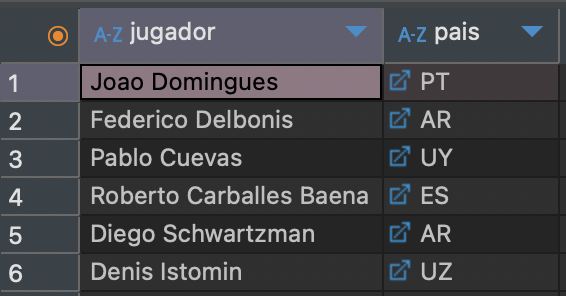
\includegraphics[width=0.35\textwidth]{fotos/q5_rel.png}
\caption{Modelo relacional Postgresql, consulta 5.}
\label{fig:q5_rel}
\end{figure}